\documentclass[10pt,paper=letter]{scrartcl}
\usepackage[alttitle]{cjquines}

\begin{document}

\title{VCSMS PRIME}
\subtitle{Program for Inducing Mathematical Excellence}
\author{Week 1 Homework}
\date{Due September 20, 2017}

\maketitle
\setlength{\unitlength}{1in}
\begin{picture}(0,0)
  \put(5.5,0.5){\hbox{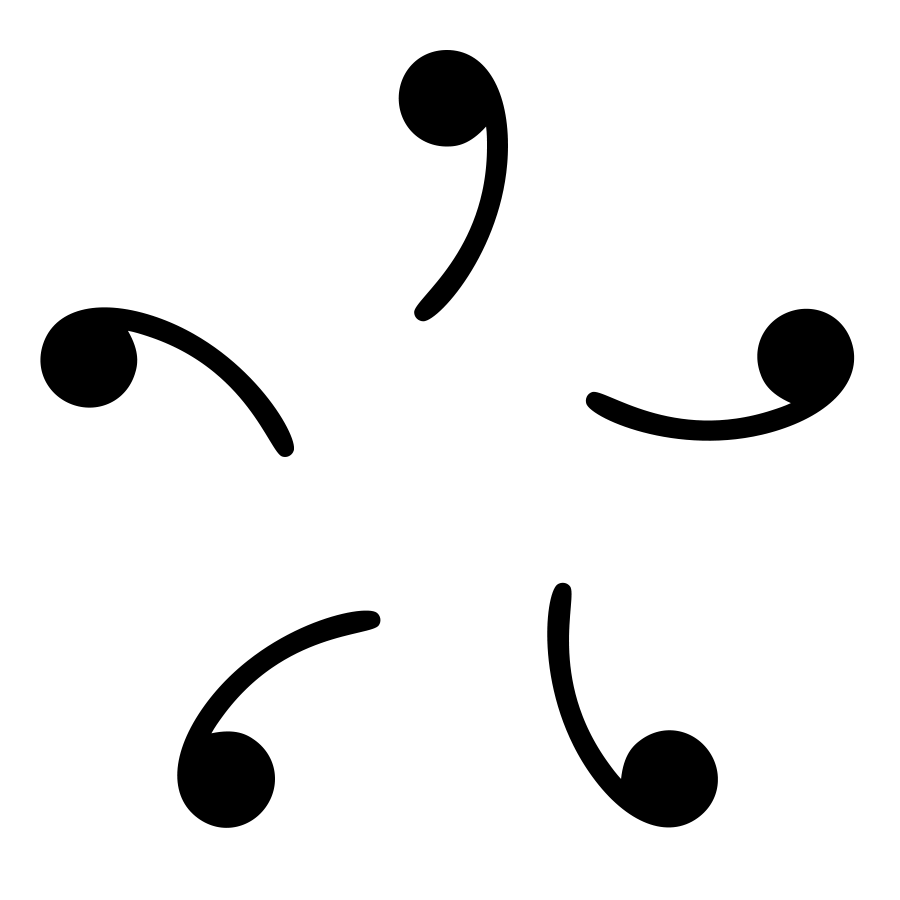
\includegraphics[width=0.9in]{logo.png}}}
\end{picture}
\vspace{-3.5em}

\subsubsection*{Homework}

Each person is assigned two sets based on their problem-solving level. For the first set assigned to you, you only need to submit your answers. For the second set, you must submit \emph{neat and orderly} solutions for each problem. Write your answers on short bond paper, write your name, and leave margins. 

Problems refer to VCSMS PRIME 2016, on \url{http://cjquines.com/files/prime.pdf}, which is also posted in our Facebook group. For example, ``\textbf{S9}: Circles 3--5, 7'' means problems 3, 4, 5 and 7 in the Circles section of PRIME 2016 session 9.

Due on Week 1 due date: Wednesday, September 20. 

\begin{description}
  \item [Set A] (13) \textbf{S1}: Domain and Range 5; Logarithms 1--2; Exponents 1--2; Value-finding 1.\\ \textbf{S7}: Angles 1; Areas 1--3. \textbf{S8}: Surds 1--3.
  \item [Set B] (15) \textbf{S1}: Domain and Range 6--7; Logarithms 3--6; Exponents 3--4; Floor, ceiling, fractional 1.\\ \textbf{S5}: Equations 7. \textbf{S7}: Angles 2--3; Areas 4--5. \textbf{S8}: Surds 4.
  \item [Set C] (16) \textbf{S1}: More logarithms: 1--2, 6--7; Floor, ceiling, fractional 2; Value-finding 2--3; Cauchy functional equation 1--3. \textbf{S5}: Equations 8. \textbf{S7}: Angles 4; Areas 6--8. \textbf{S8}: Surds 5.
  \item [Set D] (14) \textbf{S1}: More logarithms: 3--5; Floor, ceiling, fractional 3; Other functional equations 1--5.\\ \textbf{S7}: Angles 5; Areas 9--11. \textbf{S8}: Surds 6.
\end{description}

\subsubsection*{Additional problems}

These problems are optional. They range from easy to very hard.

\begin{enumerate}
  \item $ABC$ is an isosceles triangle such that $AC = BC$. $CBD$ is an isosceles triangle such that $CB = DB$. $A$ and $D$ are on the same side of line $BC$, and segments $BD$ and $AC$ intersect at a right angle. If $\angle A = 57\dg$, what is $\angle D$?

  \item Quadrilateral $CFDE$ is inscribed in a circle with center $O$, which lies on segment $CD$. Lines $CE$ and $DF$ intersect at $A$ and lines $DE$ and $CF$ intersect at $B$. If $\angle EAD = 40\dg$ and minor arc $ED$ measures $40\dg$, find $m\angle DAB$.

  \item Two equilateral triangles $ABC$ and $ADE$ are drawn, both with side length $4$, such that segments $DE$ and $BC$ intersect and $AD$ and $BC$ are perpendicular. Find the area of the region common to both triangles.
\end{enumerate}

\noindent\begin{minipage}{.70\textwidth}
  \begin{enumerate}
    \item[4.] Pentagon $ABCDE$ with side lengths $AB = BC = CD = 10, DE = 16, EA = 12$ is inscribed in a circle. If $\angle DEA = 90\dg$, find its area.

    \item[5.] (Mathira 2017) In the figure to the right, the nine circles all have radius $1$ and adjacent circles are either externally tangent or pass through each others' centers. Find the area of the shaded region.

    \item[6.] (AII2) Let $BH$ be the altitude from the vertex $B$ to the side $AC$ of an acute-angled triangle $ABC$. Let $D$ and $E$ be the midpoints of $AB$ and $AC$, respectively, and $F$ the reflection of $H$ across the line segment $ED$. Prove that the line $BF$ passes through the circumcenter of $\triangle ABC$.
  \end{enumerate}
\end{minipage}
\begin{minipage}{.32\textwidth}
  \begin{center}
  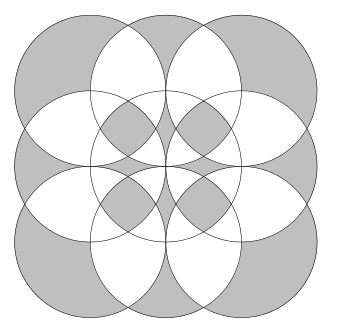
\includegraphics[width=.90\textwidth]{w1math.png}
  \end{center}
\end{minipage}

\end{document}
